
\documentclass{article} % For LaTeX2e
\usepackage{iclr2024_conference,times}

% Optional math commands from https://github.com/goodfeli/dlbook_notation.
%%%%% NEW MATH DEFINITIONS %%%%%

\usepackage{amsmath,amsfonts,bm}

% Mark sections of captions for referring to divisions of figures
\newcommand{\figleft}{{\em (Left)}}
\newcommand{\figcenter}{{\em (Center)}}
\newcommand{\figright}{{\em (Right)}}
\newcommand{\figtop}{{\em (Top)}}
\newcommand{\figbottom}{{\em (Bottom)}}
\newcommand{\captiona}{{\em (a)}}
\newcommand{\captionb}{{\em (b)}}
\newcommand{\captionc}{{\em (c)}}
\newcommand{\captiond}{{\em (d)}}

% Highlight a newly defined term
\newcommand{\newterm}[1]{{\bf #1}}


% Figure reference, lower-case.
\def\figref#1{figure~\ref{#1}}
% Figure reference, capital. For start of sentence
\def\Figref#1{Figure~\ref{#1}}
\def\twofigref#1#2{figures \ref{#1} and \ref{#2}}
\def\quadfigref#1#2#3#4{figures \ref{#1}, \ref{#2}, \ref{#3} and \ref{#4}}
% Section reference, lower-case.
\def\secref#1{section~\ref{#1}}
% Section reference, capital.
\def\Secref#1{Section~\ref{#1}}
% Reference to two sections.
\def\twosecrefs#1#2{sections \ref{#1} and \ref{#2}}
% Reference to three sections.
\def\secrefs#1#2#3{sections \ref{#1}, \ref{#2} and \ref{#3}}
% Reference to an equation, lower-case.
\def\eqref#1{equation~\ref{#1}}
% Reference to an equation, upper case
\def\Eqref#1{Equation~\ref{#1}}
% A raw reference to an equation---avoid using if possible
\def\plaineqref#1{\ref{#1}}
% Reference to a chapter, lower-case.
\def\chapref#1{chapter~\ref{#1}}
% Reference to an equation, upper case.
\def\Chapref#1{Chapter~\ref{#1}}
% Reference to a range of chapters
\def\rangechapref#1#2{chapters\ref{#1}--\ref{#2}}
% Reference to an algorithm, lower-case.
\def\algref#1{algorithm~\ref{#1}}
% Reference to an algorithm, upper case.
\def\Algref#1{Algorithm~\ref{#1}}
\def\twoalgref#1#2{algorithms \ref{#1} and \ref{#2}}
\def\Twoalgref#1#2{Algorithms \ref{#1} and \ref{#2}}
% Reference to a part, lower case
\def\partref#1{part~\ref{#1}}
% Reference to a part, upper case
\def\Partref#1{Part~\ref{#1}}
\def\twopartref#1#2{parts \ref{#1} and \ref{#2}}

\def\ceil#1{\lceil #1 \rceil}
\def\floor#1{\lfloor #1 \rfloor}
\def\1{\bm{1}}
\newcommand{\train}{\mathcal{D}}
\newcommand{\valid}{\mathcal{D_{\mathrm{valid}}}}
\newcommand{\test}{\mathcal{D_{\mathrm{test}}}}

\def\eps{{\epsilon}}


% Random variables
\def\reta{{\textnormal{$\eta$}}}
\def\ra{{\textnormal{a}}}
\def\rb{{\textnormal{b}}}
\def\rc{{\textnormal{c}}}
\def\rd{{\textnormal{d}}}
\def\re{{\textnormal{e}}}
\def\rf{{\textnormal{f}}}
\def\rg{{\textnormal{g}}}
\def\rh{{\textnormal{h}}}
\def\ri{{\textnormal{i}}}
\def\rj{{\textnormal{j}}}
\def\rk{{\textnormal{k}}}
\def\rl{{\textnormal{l}}}
% rm is already a command, just don't name any random variables m
\def\rn{{\textnormal{n}}}
\def\ro{{\textnormal{o}}}
\def\rp{{\textnormal{p}}}
\def\rq{{\textnormal{q}}}
\def\rr{{\textnormal{r}}}
\def\rs{{\textnormal{s}}}
\def\rt{{\textnormal{t}}}
\def\ru{{\textnormal{u}}}
\def\rv{{\textnormal{v}}}
\def\rw{{\textnormal{w}}}
\def\rx{{\textnormal{x}}}
\def\ry{{\textnormal{y}}}
\def\rz{{\textnormal{z}}}

% Random vectors
\def\rvepsilon{{\mathbf{\epsilon}}}
\def\rvtheta{{\mathbf{\theta}}}
\def\rva{{\mathbf{a}}}
\def\rvb{{\mathbf{b}}}
\def\rvc{{\mathbf{c}}}
\def\rvd{{\mathbf{d}}}
\def\rve{{\mathbf{e}}}
\def\rvf{{\mathbf{f}}}
\def\rvg{{\mathbf{g}}}
\def\rvh{{\mathbf{h}}}
\def\rvu{{\mathbf{i}}}
\def\rvj{{\mathbf{j}}}
\def\rvk{{\mathbf{k}}}
\def\rvl{{\mathbf{l}}}
\def\rvm{{\mathbf{m}}}
\def\rvn{{\mathbf{n}}}
\def\rvo{{\mathbf{o}}}
\def\rvp{{\mathbf{p}}}
\def\rvq{{\mathbf{q}}}
\def\rvr{{\mathbf{r}}}
\def\rvs{{\mathbf{s}}}
\def\rvt{{\mathbf{t}}}
\def\rvu{{\mathbf{u}}}
\def\rvv{{\mathbf{v}}}
\def\rvw{{\mathbf{w}}}
\def\rvx{{\mathbf{x}}}
\def\rvy{{\mathbf{y}}}
\def\rvz{{\mathbf{z}}}

% Elements of random vectors
\def\erva{{\textnormal{a}}}
\def\ervb{{\textnormal{b}}}
\def\ervc{{\textnormal{c}}}
\def\ervd{{\textnormal{d}}}
\def\erve{{\textnormal{e}}}
\def\ervf{{\textnormal{f}}}
\def\ervg{{\textnormal{g}}}
\def\ervh{{\textnormal{h}}}
\def\ervi{{\textnormal{i}}}
\def\ervj{{\textnormal{j}}}
\def\ervk{{\textnormal{k}}}
\def\ervl{{\textnormal{l}}}
\def\ervm{{\textnormal{m}}}
\def\ervn{{\textnormal{n}}}
\def\ervo{{\textnormal{o}}}
\def\ervp{{\textnormal{p}}}
\def\ervq{{\textnormal{q}}}
\def\ervr{{\textnormal{r}}}
\def\ervs{{\textnormal{s}}}
\def\ervt{{\textnormal{t}}}
\def\ervu{{\textnormal{u}}}
\def\ervv{{\textnormal{v}}}
\def\ervw{{\textnormal{w}}}
\def\ervx{{\textnormal{x}}}
\def\ervy{{\textnormal{y}}}
\def\ervz{{\textnormal{z}}}

% Random matrices
\def\rmA{{\mathbf{A}}}
\def\rmB{{\mathbf{B}}}
\def\rmC{{\mathbf{C}}}
\def\rmD{{\mathbf{D}}}
\def\rmE{{\mathbf{E}}}
\def\rmF{{\mathbf{F}}}
\def\rmG{{\mathbf{G}}}
\def\rmH{{\mathbf{H}}}
\def\rmI{{\mathbf{I}}}
\def\rmJ{{\mathbf{J}}}
\def\rmK{{\mathbf{K}}}
\def\rmL{{\mathbf{L}}}
\def\rmM{{\mathbf{M}}}
\def\rmN{{\mathbf{N}}}
\def\rmO{{\mathbf{O}}}
\def\rmP{{\mathbf{P}}}
\def\rmQ{{\mathbf{Q}}}
\def\rmR{{\mathbf{R}}}
\def\rmS{{\mathbf{S}}}
\def\rmT{{\mathbf{T}}}
\def\rmU{{\mathbf{U}}}
\def\rmV{{\mathbf{V}}}
\def\rmW{{\mathbf{W}}}
\def\rmX{{\mathbf{X}}}
\def\rmY{{\mathbf{Y}}}
\def\rmZ{{\mathbf{Z}}}

% Elements of random matrices
\def\ermA{{\textnormal{A}}}
\def\ermB{{\textnormal{B}}}
\def\ermC{{\textnormal{C}}}
\def\ermD{{\textnormal{D}}}
\def\ermE{{\textnormal{E}}}
\def\ermF{{\textnormal{F}}}
\def\ermG{{\textnormal{G}}}
\def\ermH{{\textnormal{H}}}
\def\ermI{{\textnormal{I}}}
\def\ermJ{{\textnormal{J}}}
\def\ermK{{\textnormal{K}}}
\def\ermL{{\textnormal{L}}}
\def\ermM{{\textnormal{M}}}
\def\ermN{{\textnormal{N}}}
\def\ermO{{\textnormal{O}}}
\def\ermP{{\textnormal{P}}}
\def\ermQ{{\textnormal{Q}}}
\def\ermR{{\textnormal{R}}}
\def\ermS{{\textnormal{S}}}
\def\ermT{{\textnormal{T}}}
\def\ermU{{\textnormal{U}}}
\def\ermV{{\textnormal{V}}}
\def\ermW{{\textnormal{W}}}
\def\ermX{{\textnormal{X}}}
\def\ermY{{\textnormal{Y}}}
\def\ermZ{{\textnormal{Z}}}

% Vectors
\def\vzero{{\bm{0}}}
\def\vone{{\bm{1}}}
\def\vmu{{\bm{\mu}}}
\def\vtheta{{\bm{\theta}}}
\def\va{{\bm{a}}}
\def\vb{{\bm{b}}}
\def\vc{{\bm{c}}}
\def\vd{{\bm{d}}}
\def\ve{{\bm{e}}}
\def\vf{{\bm{f}}}
\def\vg{{\bm{g}}}
\def\vh{{\bm{h}}}
\def\vi{{\bm{i}}}
\def\vj{{\bm{j}}}
\def\vk{{\bm{k}}}
\def\vl{{\bm{l}}}
\def\vm{{\bm{m}}}
\def\vn{{\bm{n}}}
\def\vo{{\bm{o}}}
\def\vp{{\bm{p}}}
\def\vq{{\bm{q}}}
\def\vr{{\bm{r}}}
\def\vs{{\bm{s}}}
\def\vt{{\bm{t}}}
\def\vu{{\bm{u}}}
\def\vv{{\bm{v}}}
\def\vw{{\bm{w}}}
\def\vx{{\bm{x}}}
\def\vy{{\bm{y}}}
\def\vz{{\bm{z}}}

% Elements of vectors
\def\evalpha{{\alpha}}
\def\evbeta{{\beta}}
\def\evepsilon{{\epsilon}}
\def\evlambda{{\lambda}}
\def\evomega{{\omega}}
\def\evmu{{\mu}}
\def\evpsi{{\psi}}
\def\evsigma{{\sigma}}
\def\evtheta{{\theta}}
\def\eva{{a}}
\def\evb{{b}}
\def\evc{{c}}
\def\evd{{d}}
\def\eve{{e}}
\def\evf{{f}}
\def\evg{{g}}
\def\evh{{h}}
\def\evi{{i}}
\def\evj{{j}}
\def\evk{{k}}
\def\evl{{l}}
\def\evm{{m}}
\def\evn{{n}}
\def\evo{{o}}
\def\evp{{p}}
\def\evq{{q}}
\def\evr{{r}}
\def\evs{{s}}
\def\evt{{t}}
\def\evu{{u}}
\def\evv{{v}}
\def\evw{{w}}
\def\evx{{x}}
\def\evy{{y}}
\def\evz{{z}}

% Matrix
\def\mA{{\bm{A}}}
\def\mB{{\bm{B}}}
\def\mC{{\bm{C}}}
\def\mD{{\bm{D}}}
\def\mE{{\bm{E}}}
\def\mF{{\bm{F}}}
\def\mG{{\bm{G}}}
\def\mH{{\bm{H}}}
\def\mI{{\bm{I}}}
\def\mJ{{\bm{J}}}
\def\mK{{\bm{K}}}
\def\mL{{\bm{L}}}
\def\mM{{\bm{M}}}
\def\mN{{\bm{N}}}
\def\mO{{\bm{O}}}
\def\mP{{\bm{P}}}
\def\mQ{{\bm{Q}}}
\def\mR{{\bm{R}}}
\def\mS{{\bm{S}}}
\def\mT{{\bm{T}}}
\def\mU{{\bm{U}}}
\def\mV{{\bm{V}}}
\def\mW{{\bm{W}}}
\def\mX{{\bm{X}}}
\def\mY{{\bm{Y}}}
\def\mZ{{\bm{Z}}}
\def\mBeta{{\bm{\beta}}}
\def\mPhi{{\bm{\Phi}}}
\def\mLambda{{\bm{\Lambda}}}
\def\mSigma{{\bm{\Sigma}}}

% Tensor
\DeclareMathAlphabet{\mathsfit}{\encodingdefault}{\sfdefault}{m}{sl}
\SetMathAlphabet{\mathsfit}{bold}{\encodingdefault}{\sfdefault}{bx}{n}
\newcommand{\tens}[1]{\bm{\mathsfit{#1}}}
\def\tA{{\tens{A}}}
\def\tB{{\tens{B}}}
\def\tC{{\tens{C}}}
\def\tD{{\tens{D}}}
\def\tE{{\tens{E}}}
\def\tF{{\tens{F}}}
\def\tG{{\tens{G}}}
\def\tH{{\tens{H}}}
\def\tI{{\tens{I}}}
\def\tJ{{\tens{J}}}
\def\tK{{\tens{K}}}
\def\tL{{\tens{L}}}
\def\tM{{\tens{M}}}
\def\tN{{\tens{N}}}
\def\tO{{\tens{O}}}
\def\tP{{\tens{P}}}
\def\tQ{{\tens{Q}}}
\def\tR{{\tens{R}}}
\def\tS{{\tens{S}}}
\def\tT{{\tens{T}}}
\def\tU{{\tens{U}}}
\def\tV{{\tens{V}}}
\def\tW{{\tens{W}}}
\def\tX{{\tens{X}}}
\def\tY{{\tens{Y}}}
\def\tZ{{\tens{Z}}}


% Graph
\def\gA{{\mathcal{A}}}
\def\gB{{\mathcal{B}}}
\def\gC{{\mathcal{C}}}
\def\gD{{\mathcal{D}}}
\def\gE{{\mathcal{E}}}
\def\gF{{\mathcal{F}}}
\def\gG{{\mathcal{G}}}
\def\gH{{\mathcal{H}}}
\def\gI{{\mathcal{I}}}
\def\gJ{{\mathcal{J}}}
\def\gK{{\mathcal{K}}}
\def\gL{{\mathcal{L}}}
\def\gM{{\mathcal{M}}}
\def\gN{{\mathcal{N}}}
\def\gO{{\mathcal{O}}}
\def\gP{{\mathcal{P}}}
\def\gQ{{\mathcal{Q}}}
\def\gR{{\mathcal{R}}}
\def\gS{{\mathcal{S}}}
\def\gT{{\mathcal{T}}}
\def\gU{{\mathcal{U}}}
\def\gV{{\mathcal{V}}}
\def\gW{{\mathcal{W}}}
\def\gX{{\mathcal{X}}}
\def\gY{{\mathcal{Y}}}
\def\gZ{{\mathcal{Z}}}

% Sets
\def\sA{{\mathbb{A}}}
\def\sB{{\mathbb{B}}}
\def\sC{{\mathbb{C}}}
\def\sD{{\mathbb{D}}}
% Don't use a set called E, because this would be the same as our symbol
% for expectation.
\def\sF{{\mathbb{F}}}
\def\sG{{\mathbb{G}}}
\def\sH{{\mathbb{H}}}
\def\sI{{\mathbb{I}}}
\def\sJ{{\mathbb{J}}}
\def\sK{{\mathbb{K}}}
\def\sL{{\mathbb{L}}}
\def\sM{{\mathbb{M}}}
\def\sN{{\mathbb{N}}}
\def\sO{{\mathbb{O}}}
\def\sP{{\mathbb{P}}}
\def\sQ{{\mathbb{Q}}}
\def\sR{{\mathbb{R}}}
\def\sS{{\mathbb{S}}}
\def\sT{{\mathbb{T}}}
\def\sU{{\mathbb{U}}}
\def\sV{{\mathbb{V}}}
\def\sW{{\mathbb{W}}}
\def\sX{{\mathbb{X}}}
\def\sY{{\mathbb{Y}}}
\def\sZ{{\mathbb{Z}}}

% Entries of a matrix
\def\emLambda{{\Lambda}}
\def\emA{{A}}
\def\emB{{B}}
\def\emC{{C}}
\def\emD{{D}}
\def\emE{{E}}
\def\emF{{F}}
\def\emG{{G}}
\def\emH{{H}}
\def\emI{{I}}
\def\emJ{{J}}
\def\emK{{K}}
\def\emL{{L}}
\def\emM{{M}}
\def\emN{{N}}
\def\emO{{O}}
\def\emP{{P}}
\def\emQ{{Q}}
\def\emR{{R}}
\def\emS{{S}}
\def\emT{{T}}
\def\emU{{U}}
\def\emV{{V}}
\def\emW{{W}}
\def\emX{{X}}
\def\emY{{Y}}
\def\emZ{{Z}}
\def\emSigma{{\Sigma}}

% entries of a tensor
% Same font as tensor, without \bm wrapper
\newcommand{\etens}[1]{\mathsfit{#1}}
\def\etLambda{{\etens{\Lambda}}}
\def\etA{{\etens{A}}}
\def\etB{{\etens{B}}}
\def\etC{{\etens{C}}}
\def\etD{{\etens{D}}}
\def\etE{{\etens{E}}}
\def\etF{{\etens{F}}}
\def\etG{{\etens{G}}}
\def\etH{{\etens{H}}}
\def\etI{{\etens{I}}}
\def\etJ{{\etens{J}}}
\def\etK{{\etens{K}}}
\def\etL{{\etens{L}}}
\def\etM{{\etens{M}}}
\def\etN{{\etens{N}}}
\def\etO{{\etens{O}}}
\def\etP{{\etens{P}}}
\def\etQ{{\etens{Q}}}
\def\etR{{\etens{R}}}
\def\etS{{\etens{S}}}
\def\etT{{\etens{T}}}
\def\etU{{\etens{U}}}
\def\etV{{\etens{V}}}
\def\etW{{\etens{W}}}
\def\etX{{\etens{X}}}
\def\etY{{\etens{Y}}}
\def\etZ{{\etens{Z}}}

% The true underlying data generating distribution
\newcommand{\pdata}{p_{\rm{data}}}
% The empirical distribution defined by the training set
\newcommand{\ptrain}{\hat{p}_{\rm{data}}}
\newcommand{\Ptrain}{\hat{P}_{\rm{data}}}
% The model distribution
\newcommand{\pmodel}{p_{\rm{model}}}
\newcommand{\Pmodel}{P_{\rm{model}}}
\newcommand{\ptildemodel}{\tilde{p}_{\rm{model}}}
% Stochastic autoencoder distributions
\newcommand{\pencode}{p_{\rm{encoder}}}
\newcommand{\pdecode}{p_{\rm{decoder}}}
\newcommand{\precons}{p_{\rm{reconstruct}}}

\newcommand{\laplace}{\mathrm{Laplace}} % Laplace distribution

\newcommand{\E}{\mathbb{E}}
\newcommand{\Ls}{\mathcal{L}}
\newcommand{\R}{\mathbb{R}}
\newcommand{\emp}{\tilde{p}}
\newcommand{\lr}{\alpha}
\newcommand{\reg}{\lambda}
\newcommand{\rect}{\mathrm{rectifier}}
\newcommand{\softmax}{\mathrm{softmax}}
\newcommand{\sigmoid}{\sigma}
\newcommand{\softplus}{\zeta}
\newcommand{\KL}{D_{\mathrm{KL}}}
\newcommand{\Var}{\mathrm{Var}}
\newcommand{\standarderror}{\mathrm{SE}}
\newcommand{\Cov}{\mathrm{Cov}}
% Wolfram Mathworld says $L^2$ is for function spaces and $\ell^2$ is for vectors
% But then they seem to use $L^2$ for vectors throughout the site, and so does
% wikipedia.
\newcommand{\normlzero}{L^0}
\newcommand{\normlone}{L^1}
\newcommand{\normltwo}{L^2}
\newcommand{\normlp}{L^p}
\newcommand{\normmax}{L^\infty}

\newcommand{\parents}{Pa} % See usage in notation.tex. Chosen to match Daphne's book.

\DeclareMathOperator*{\argmax}{arg\,max}
\DeclareMathOperator*{\argmin}{arg\,min}

\DeclareMathOperator{\sign}{sign}
\DeclareMathOperator{\Tr}{Tr}
\let\ab\allowbreak


\usepackage{chngpage}
\usepackage{booktabs}
\usepackage{graphicx}
\usepackage{hyperref}
\usepackage{url}


\title{Interpretable Risk Minimization}

% Authors must not appear in the submitted version. They should be hidden
% as long as the \iclrfinalcopy macro remains commented out below.
% Non-anonymous submissions will be rejected without review.

\author{Jinen Setpal (PUID 0033541028) \\
Department of Computer Science \\
Purdue University \\
West Lafeyette, IN 47906, USA \\
\texttt{jsetpal@cs.purdue.edu}
}

% The \author macro works with any number of authors. There are two commands
% used to separate the names and addresses of multiple authors: \And and \AND.
%
% Using \And between authors leaves it to \LaTeX{} to determine where to break
% the lines. Using \AND forces a linebreak at that point. So, if \LaTeX{}
% puts 3 of 4 authors names on the first line, and the last on the second
% line, try using \AND instead of \And before the third author name.

\newcommand{\fix}{\marginpar{FIX}}
\newcommand{\new}{\marginpar{NEW}}

% \iclrfinalcopy % Uncomment for camera-ready version, but NOT for submission.
\begin{document}

\maketitle

\section{Introduction}
\label{intro}

A few critical assumptions are often made by machine learning researchers and practitioners training neural networks. Specifically; an optimal neural network is robust to an unseen sample on the following primary assumptions: a) the chosen architecture is expressive enough to generalize to the data, and b) their dataset is a representative sample of the global distribution. We focus our discussion on this second assumption.

In most cases, especially in restricted or niche domains -- it is incredibly rare to find and even harder to verify a truly representative dataset. Additionally, neural networks are fundamentally associative in nature. That, alongside the overparameterized nature of models with regularizers that promote using fewer parameters often results in model posteriors that either overfit to data or learn correlations within the dataset \citep{kanal1964recognition}.

Researchers today are generally aware of this. To ensure that models do not fit to spurious correlations, a significant body of research explores techniques for \textit{machine interpretability} -- the degree to which a human can understand the cause of a decision \citep{molnar2020interpretable}.

Broadly, interpretability within machine learning is classified into two distinct types: post-hoc interpretability \citep{madsen2022post} and intrinsic interepretability \citep{pintelas2020grey, sarkar2022framework, reddy2022causally}. Post-hoc techniques for machine interpretability include approaches that are used as ``sanity checks''; to ensure accurate convergence at the end of training, whereas intrinsic interpretability techniques include approaches that are used as part of the training regime, to guide model convergence.

The ideal objective is to ensure that the model backbone, $\Gamma(x; {\bf W_\Gamma})$, learns an environment-invariant representation of the target, ensuring that the downstream MLP can perform the task without interference from correlating factors. For this work, we limit the scope of the overall objective to maximizing the worst-group performance. Group-split performance of the dataset refers to the accuracy of the model split by the specific environment in which the target is present. We discuss this in further detail under Section \ref{dataset}. Ensuring equal group-split performance within datasets is also a proposed definition of fairness. Therefore, an additional loosely defined-objective would be ensuring fairer representations of the dataset targets.

This work establishes a proof-of-concept that is able to leverage post-hoc interpretability techniques as part of the training process. By mathematically formalizing inductive loss functions that exploit implicit shared knowledge within the dataset, we aim to update the search space of the model to that of a convex optimization problem; following which backpropagration using elementary optimizers such as Stochastic Gradient Descent \citep{amari1993backpropagation} are able to obtain the global cost minima, establishing an interpretable basis for training neural networks.

\section{Dataset}
\label{dataset}

For this task, we use leverage the \textbf{Waterbirds} \citep{sagawa2019distributionally} dataset to test the proposed approach. The dataset contains two classes: landbirds and waterbirds. This is a binary classification task. Crucially, these landbirds and waterbirds are placed in two distinct environments. There are, therefore four different ``types'' of images: \textbf{landbirds on land}, \textbf{landbirds on water}, \textbf{waterbirds on land}, and \textbf{waterbirds on water}. These groups are present in equal proportions during testing. During training, there is a group imbalance; with most samples of landbirds being on land, and most samples of waterbirds being on water, introducing out-of-distribution testing.

Part of the research objective is to perform an ablation study using the proposed interpretable training techniques against the empirical risk minimization methods presented in \citep{liu2021just}, which is another reason for using the \textbf{Waterbirds} dataset.

The proposed approach has also been tested on a manually modified version of the \textbf{CALTECH-256} \citep{griffin2007caltech} dataset. It must be noted that this was mostly to test the concept, and while it worked well to simulate the target situation, it is not a reliable benchmark. The \textbf{Waterbirds} dataset is a known benchmark for out-of-distribution generalization, and solves this.

\section{Methodology}

We establish the approach as a bi-leveled optimization problem. Similar to \citep{arjovsky2019invariant}, $ D_E := \{(x^e_i, y^e_i)\}_{i=1}^{n_e} $ is the dataset consisting $E := \{e_i\}^{n_e}_{i=1}$ differing environments. Given $D_W$ s.t. $W \subset E$, our objective is to effectively predict $y_i^e \in D_U$ given $x_i^e$, where $U = E - W$.
\begin{align*}
	\text{Let } & \mathcal{X} \in \mathbb{R}^{n \times n \times c},\ \mathcal{H} \in \mathbb{R}^{l \times m}, \mathcal{Y} \subset \mathbb{R} \\
		    & \Phi : \mathcal{X} \rightarrow \mathcal{H} \rightarrow \mathcal{Y}
\end{align*}

Where $\Phi(\mathcal{X})$ is a multiheaded classifier outputting the hidden representation in addition to the classification. $\mathcal{X}$ is the input representation, $\mathcal{H}$ is an arbitrary latent representation and $\mathcal{Y}$ is the classification output. Our objective is to optimize $\Phi(x_i^e) := \{f(\Gamma(x;{\bf W_\Gamma});{\bf{W_f}})^e, h_i^e\} \approx \{y_i^e, \mu\}; \mu \in \mathbb{R}^\mathbb{N}$ using dataset specific cost functions defined within Section \ref{cam}.

\subsection{Architecture}

\begin{figure}[t]
	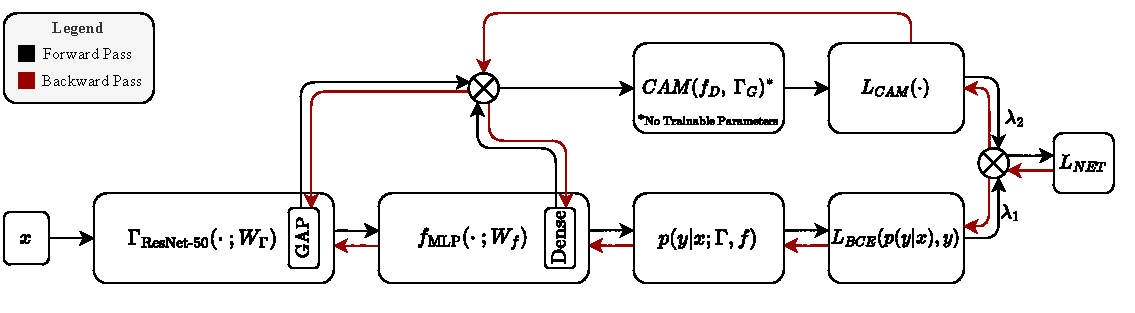
\includegraphics[width=\textwidth]{figs/architecture}
	\caption{Model architecture with highlighted backward and forward passes.}
	\label{arch}
\end{figure}

The objective of the approach was to directly compare against similar approaches to risk minimization. While any architecture can be utilized for the approach provided that a class activation mapping is obtainable, we chose to use the architecture utilized by \citep{liu2021just} for an ideal ablation study. We fine-tune the ResNet-50 backbone pre-trained on ImageNet, with a single MLP layer with softmax activation resulting in the final prediction. The architecture is as shown in Figure \ref{arch}.

The model output is multiheaded, with the actual classification along with the class activation map as output. Each head has it's own loss, a linear combination of which returns the net resultant loss. Particulars regarding hyperparameters are discussed in Section \ref{hyperparams}.

\subsubsection{Training Details}
\label{hyperparams}

\paragraph{Learning Scheduler.} The learning rates as well as loss weights are updated by the learning scheduler, split into three phases: a) bootstrapping, b) training, and c) fine-tuning. The transitions occur at $20\%$ and $80\%$ of the total epochs on which the model was trained. Since the model was trained on 30 epochs, these transitions occurred at epochs $6$ and $24$ respectively. The learning rate (LR) and loss weight (LW) splits are as follows:
\begin{itemize}
	\item[Epochs 1-5:] LR: $10^{-3}$, LW: \{BCE: $7 \times 10^{-1}$, CAM: $1$\}
	\item[Epochs 6-23:] LR: $10^{-4}$, LW: \{BCE: $8 \times 10^{-1}$, CAM: $5 \times 10^2$\}
	\item[Epochs 24-30:] LR: $10^{-6}$, LW: \{BCE: $1$, CAM: $0$\} 
\end{itemize}

\paragraph{Optimizer.} We use Stochastic Gradient Descent with momentum $\theta = 0.9$, with learning rate is updated based on the scheduler defined above.

\paragraph{DataGenerator.} The waterbirds dataset contains a minor label shift between splits, with $\text{landbird}:\text{waterbird} :: \{3.3081, 3.5075, 3.5125\}:1$, for training, validation and testing respectively. This split was not accounted for during the data generation process. However, sample stratification by class ratios for the training split was enforced, with random sampling applied for validation and testing sets.

\paragraph{Batch Size.} We used a batch size of 24, due to the memory restrictions imposed by the available compute. Most other approaches \citep{liu2021just} trained their models using a batch size of 64.

\subsection{Class Activation Mappings}
\label{cam}

Class Activation Mappings (CAMs) \citep{zhou2016learning} is a method of target localization. By obtaining the projection of weights from the final convolutional layer onto the penultimate dense layer (under the assumption that the number of convolutional filters equals the number of dense neurons), and superimposing it over the original image, we are able to obtain a heatmap of the region used for classification.

We leverage this by utilizing the implicit knowledge within our provided dataset. As an example, both the \textbf{Waterbirds} and \textbf{CALTECH-256} datasets have centred every target within their images. We evaluate the mean-squared sum of an inverted 2D Gaussian projected against the Class Activation Mapping producing the additional, self-supervised loss function. Formally, we minimize the following objective function:

\begin{align*}
	L(\Phi(x_i^e), y_i^e) &= L_{BCE}(f(\Gamma(x;{\bf W_\Gamma});{\bf W_f})_i^e, y_i^e) + L_{CAM}(h_i^e) \\
	L(\Phi(x_i^e), y_i^e) &= \frac{1}{N}\sum^N_{i=0}\sum^1_{j=0}y_i^e\log(f(\Gamma(x;{\bf W_\Gamma});{{\bf W_f}})_i^e) ) + \sum^N_{i=0}\sum^l_{j=0}\sum^m_{k=0} [(1 - e^{-j^2 - k^2}) \cdot \sigma_{\text{relu}}(h_i^{j,k})]^2
\end{align*}

A visualization of the obtained activation map for a sample spuriously correlating the background, along with the mask against which it is weakly supervised is as follows:

\begin{figure}[h]
	\centering
	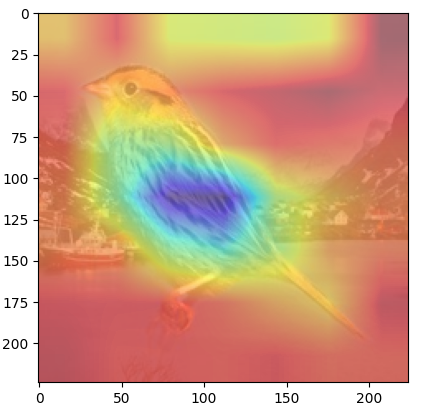
\includegraphics[width=.4\textwidth]{figs/cams.png}
	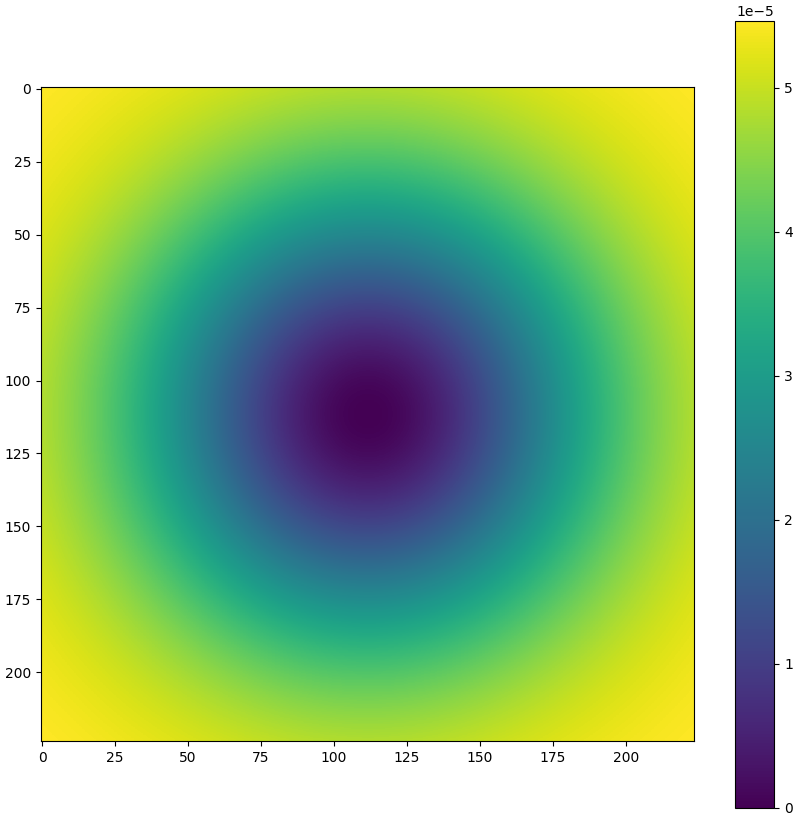
\includegraphics[width=.4\textwidth]{figs/mask.png}
\end{figure}

In this case, although the classification is accurate, the sample produces a high loss due to the fact that the background is used for basing the classification, and not the target itself. This establishes a curriculum-style approach to model optimizitation wherein intermediary layers are checkpointed and backpropagated against. To ensure that our network is unable to overfit to the gaussian projection, we combine this with transformation and translation equivariant convolutional representations, following \citep{mouli2021neural}.

\section{Related Work}

\cite{arjovsky2019invariant} presents a causal approach towards out-of-distribution generalization. The paper discusses identifying environment-invariant predictors by deriving a penalty based on the structural causal model defined in their paper.

\cite{liu2021just} uses empirical methods to achieve the same objective. The authors train an identification model that associates sample with high training losses. These are then upweighted, enabling generalization across domains. However, the primary limitation of this work is that it requires the existence of a small set of samples within a dataset. These edge cases are then highlighted. While it allows for better generalization within the sampled distribution, it does not account for samples outside the training distribution.

\cite{krueger2021out} presents a form of robust optimization over a perturbation set of extrapolated domains in addition to a simpler penalty on the variance of training risks. It is able to recover the causal mechanisms of the targets and is also resilient to covariate shift.

% add DRO

\section{Results}

As stated within Section \ref{intro}, the objective of the model was to learn a latent representation invariant to the background of the model. Since Class Activation Mappings are fundamentally a post-hoc tool, we can use them to compare the regions used for image identification. The following figure displays the class activation mappings for training run with standard ERM, and the updated CAM-based approach:

\begin{figure}[h]
	\centering
	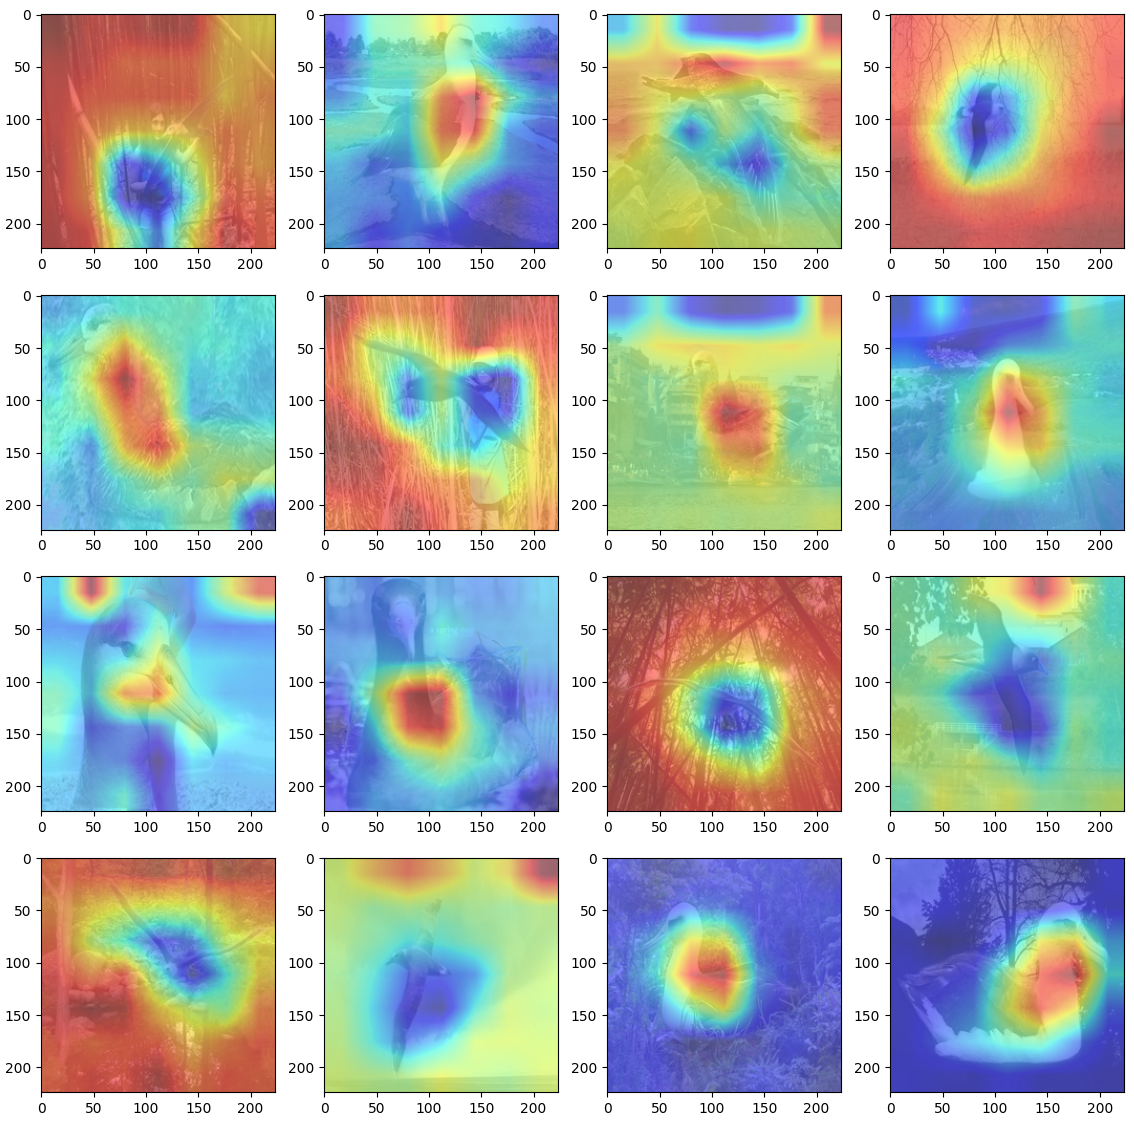
\includegraphics[width=.468\textwidth]{figs/default}
	\ \ \ \ \ \ 
	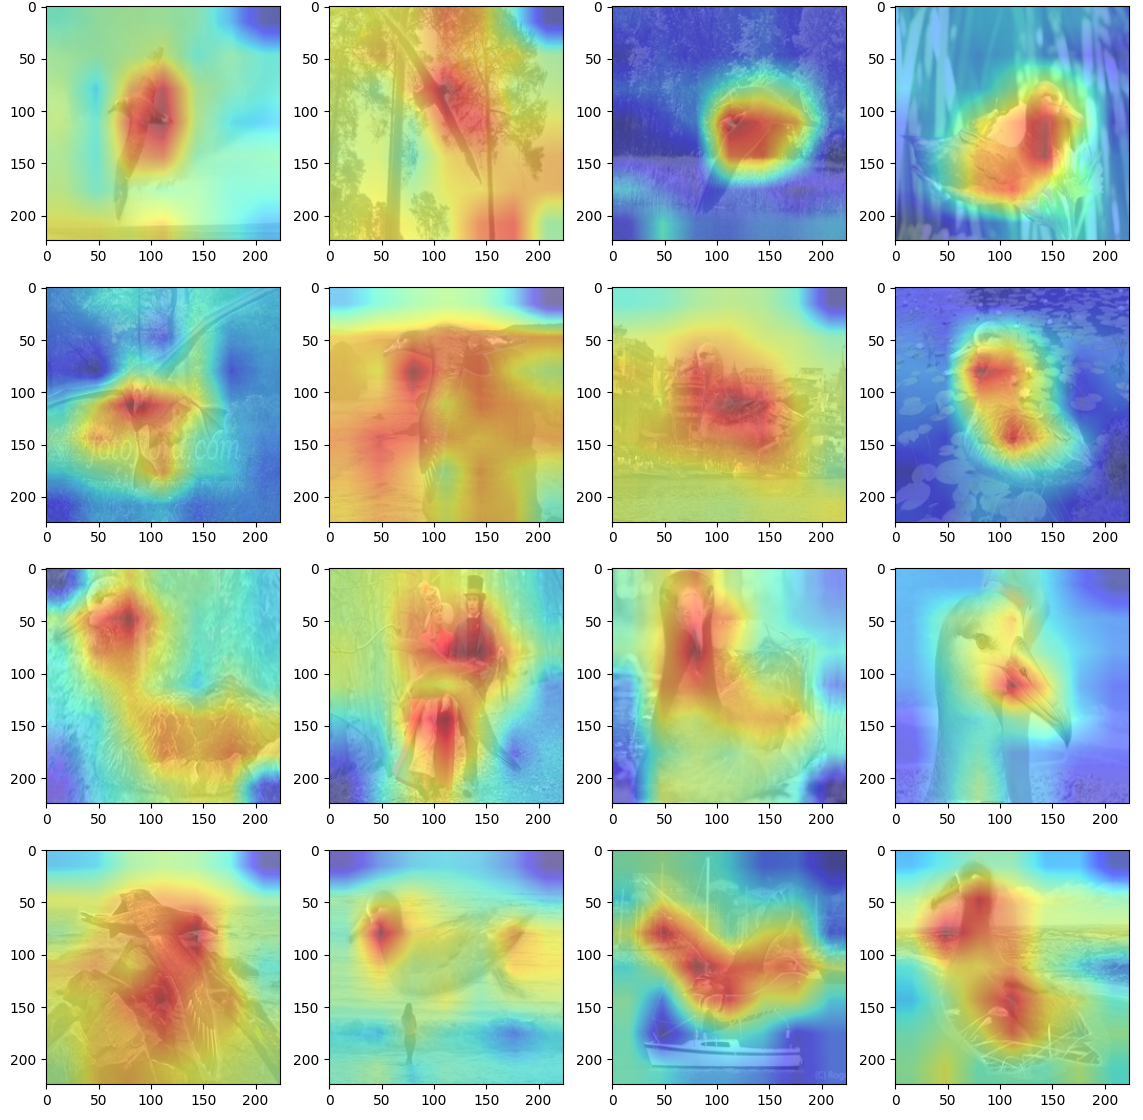
\includegraphics[width=.468\textwidth]{figs/camloss}
	\caption{(a) CAMs of evaluations trained using ERM; (b) CAMs of evaluations trained using Interpret-RM.}
\end{figure}

We observe samples in the ERM-based approach where the model places a high weightage on the background of the image, implying that shortcut learning is employed to learn the data distribution. When the same model architecture is trained using Interpret-RM, we observe that this is mitigated, as there is a higher weightage placed on the actual targets within the image.

One of the concerns during the development of the approach was that by centering the image, we could overfit the model to the inverse gaussian, and the model would only observe the center, regardless of the location of the actual target. Crucially, when we tested a model trained with the updated approach against an image translationally migrated to have the target at the edge of the image, the model was able to accurately identify the region where the target was present, and not the just focus on the center. 

There are a couple of reasons for this. First, this approach was viable due to the inbuilt mechanism for translation equviariance within convolutional neural networks. Second, and likely more important, is that the \underline{loss is a reductionist value}. The optimization algorithm does not know \textit{why} it receives a high cost for a given inference. As long as the correlation between the metric for the interpretable loss devised by the practitioner is close enough that is can weakly identify when the model is performing optimally, cost function performs as though it is a background/foreground identifier, even the heuristic does not universally hold. The closest minima for the model is now updated to that of the target itself, and therefore the model focuses on the target regardless of it's location during inference. However, if we over-weight the devised mask, it will overfit to the central portion of the image and will not work optimally.

We evaluate our approach against a series of state-of-the-art approaches to group minimization. Updating the table from \citep{kim2022sharpnessaware}, we report the following metrics on the \textbf{Waterbirds} dataset:

\setlength\tabcolsep{3pt}
\begin{table}[h]
	\begin{adjustwidth}{-.5in}{-.5in}  
	\begin{tabular}{c|ccc|cccc}
		\toprule
		\textbf{Method}  & \textbf{Average}  & \textbf{Group Average}   & \textbf{Worst Group}    & \textbf{LL}                         & \textbf{LW}                         & \textbf{WL}                         & \textbf{WW}               \\
		\midrule
		ERM              & 97.1              & 84.1                     & 69.8                    & 99.3 $\pm$ 0.1                      & 71.5 $\pm$ 0.5                      & 69.8 $\pm$ 0.6                      & 95.8 $\pm$ 0.2            \\
		SAM              & \textbf{97.6}     & 87.2                     & 75.5                    & 99.4 $\pm$ 0.1             & 77.5 $\pm$ 1.8                      & 75.5 $\pm$ 1.0                      & \textbf{96.4} $\pm$ \textbf{0.3}   \\
		GDRO             & 93.8              & 90.4                     & 86.5                    & 94.7 $\pm$ 0.7                      & 86.5 $\pm$ 0.7                      & 88.1 $\pm$ 0.3                      & 92.3 $\pm$ 0.3            \\
		SGDRO            & 93.1              & \textbf{90.6}            & \textbf{87.2}           & 93.8 $\pm$ 1.7                      & \textbf{87.2} $\pm$ \textbf{0.5}    & \textbf{89.3} $\pm$ \textbf{0.3}    & 92.0 $\pm$ 0.8            \\
		\midrule
		\textbf{Interpret-RM (Ours)} & 86.3              & 80.6            & 48.8           & \textbf{99.6 $\pm$ 0.1}                      & 83.7 $\pm$ 0.1    & 48.8 $\pm$ 0.1    & 90.3 $\pm$ 0.8            \\
		\bottomrule
	\end{tabular}
\end{adjustwidth}
\end{table}

We observe that our approach does not perform optimally to the target dataset. We address this in Section \ref{limitations}. 

\subsection{Limitations}
\label{limitations}

Regarding benchmark performance, we attribute it primarily to the low batch size used to train the model. We also did not perform any hyperparameter tuning, and assume improvements as a consequence. Finally, we also did not experiment with the various designs of the interpretable loss function, and do not believe the current solution is optimal for the task.

In addition, this approach fails to formally the objective function within the context of interpretability. One of the consequences for this is the naive design of the interpretable loss function. While it is able to converge towards solutions that do not use the background, it is not well balanced, and needs to often be manually tuned to ensure it is not over or under-powered.

Finally, the greatest limitation within the approach is it's lack of generalizability. It requires the dataset to contain a certain shared characteristics, that represents an inductive bias that can be mathematically applied to the dataset. For future work, the objective is to introduce generalizable metrics based on statistically observed behaviors within accurate and inaccurate activation mappings, rather than the use of hardcoded, task and dataset-specific masks to achieve a similar result.

\paragraph{Reproducibility.} The code, data, models, experiments and execution pipelines are hosted at \url{https://dagshub.com/jinensetpal/lint}. The pipeline is structured as a DAG, and can be replicated end-to-end with a single command.

\bibliography{iclr2024_conference}
\bibliographystyle{iclr2024_conference}

\end{document}
